\documentclass[a4paper,12pt]{extarticle}

%Packages:
\usepackage[utf8]{inputenc}    
\usepackage[vietnamese]{babel} 
\usepackage{graphicx}          
\usepackage{amsmath , amsfonts , amssymb , amsthm} 
\usepackage{hyperref}          
\usepackage{geometry}    
\usepackage{framed}
\usepackage{float}
\usepackage{array}
\geometry{a4paper, margin=1in}

\begin{document}
%Trang bìa
\begin{titlepage}
    \centering
    {\textbf{ĐẠI HỌC QUỐC GIA THÀNH PHỐ HỒ CHÍ MINH} \\   
    {\textbf{TRƯỜNG ĐẠI HỌC BÁCH KHOA}} \\   
    {\textbf{BỘ MÔN TOÁN ỨNG DỤNG}} \\
%Chèn logo BK    
\begin{figure}[h]
    \centering
    
\includegraphics[width=0.4\textwidth]{img/Bach khoa.png}
\end{figure}
%Title
    { \textbf{BÁO CÁO BÀI TẬP LỚN MÔN ĐẠI SỐ TUYẾN TÍNH}} \\
    \hrulefill \\}
    {\huge \textbf{Cơ sở lý thuyết của phân tích Fisherface Method và ứng dụng của phân tích SVD trong nhận diện khuôn mặt.}} \\
    \vspace{0.5cm}
    
    { \textbf{GVHD: T.S Đặng Văn Vinh}} \\
    {\textbf{Nhóm thực hiện: Nhóm 4}}
    \vspace{1cm}

\begin{tabular}{|m{1cm}|m{3cm}|m{3cm}|m{2cm}|}
\hline
STT & Họ và đệm  & Tên &  MSSV \\ \hline
1 & Nguyễn Thái & Hưng & 0000000 \\ \hline
\end{tabular}
\vspace{5cm} \\
\textbf{Thành phố Hồ Chí Minh, tháng 11 năm 2024}
\end{titlepage}
%Mục lục
\tableofcontents
\newpage

%Chapter 1 Lời nói đầu
\section{Mở đầu} 
\subsection{Lời cảm ơn}
Nhóm em xin gửi lời cảm ơn chân thành nhất đến thầy Đặng Văn Vinh đã hướng dẫn và hỗ trợ trong quá trình thực hiện bài báo cáo bài tập lớn . Bài báo cáo đã giúp chúng em hiểu sâu hơn về các khái niệm và nguyên lý liên quan đến đề tài của chúng em nói riêng và bộ môn Đại số tuyến tính nói chung. Ngoài ra còn giúp chúng em phát triển kỹ năng nghiên cứu và trình bày một bài báo cáo khoa học.\\
Chúng em rất trân trọng đến sự quan tâm và hỗ trợ của thầy trong quá trình học và thực hiện đề tài.Mong rằng bài báo cáo lần này của chúng em đã đáp ứng được những kỳ vọng và yêu cầu của thầy.
\subsection{Giới thiệu sơ lược về đề tài}
Nhận diện khuôn mặt là một trong những công nghệ quan trọng và được ứng dụng rộng rãi trong đời sống hiện đại. Từ các hệ thống an ninh đến giao diện tương tác người-máy, khả năng nhận diện khuôn mặt tự động đã tạo ra những bước tiến lớn trong nhiều lĩnh vực. Trong bối cảnh đó, việc ứng dụng các công cụ toán học mạnh mẽ như phân tích giá trị kỳ dị (Singular Value Decomposition - SVD) và Fisherface Method mang lại hiệu quả cao trong việc xử lý và phân loại dữ liệu khuôn mặt. \\
Phân tích SVD là một kỹ thuật giảm chiều dữ liệu phổ biến, giúp tối ưu hóa việc trích xuất các đặc trưng quan trọng từ dữ liệu hình ảnh. Khi kết hợp với Fisherface Method, dựa trên phân tích tuyến tính phân biệt (Linear Discriminant Analysis - LDA), hệ thống nhận diện khuôn mặt có thể phân loại chính xác hơn nhờ tăng cường khả năng phân biệt giữa các đối tượng. Python, với các thư viện hỗ trợ mạnh mẽ như NumPy, OpenCV và scikit-learn, mang lại sự linh hoạt trong triển khai thuật toán nhận diện khuôn mặt, từ việc trích xuất đặc trưng đến đánh giá hiệu quả phân loại.\\
Trong nghiên cứu này, phân tích SVD sẽ được ứng dụng để trích xuất các đặc trưng khuôn mặt từ hình ảnh xám và tối ưu hóa quá trình phân loại. Các kết quả thu được sẽ minh họa cách tiếp cận toán học trong việc giải quyết bài toán nhận diện khuôn mặt với dữ liệu giả lập hoặc thực tế.
%Chapter 2 Cơ sở lý thuyết
\section{Cơ sở lý thuyết}
%Phân tích SVD
\subsection{Phân tích giá trị kì dị (Singular Value Decomposition - SVD)}
Phân tích giá trị kỳ dị (SVD) là một công cụ toán học mạnh mẽ trong việc phân tích và xử lý ma trận, được ứng dụng rộng rãi trong các lĩnh vực như học máy, xử lý ảnh và khai phá dữ liệu. Đối với một ma trận A có kích thước m×n, SVD cho phép phân rã ma trận này thành ba ma trận thành phần:
\[
A = U \Sigma V^T
\]
Trong đó:
\begin{itemize}
    \item U: Ma trận trực giao kích thước m×m, chứa các vector riêng của $AA^T$ , đại diện cho không gian hàng của A.
    \item V: Ma trận trực giao kích thước n×n, chứa các vector riêng của $A^TA$ , đại diện cho không gian cột của A.
    \item $\Sigma$: Ma trận đường chéo m×n, chứa các giá trị kỳ dị (singular values) sắp xếp giảm dần ($\sigma _1  \geq \sigma _ 2 \geq ... \geq \sigma _k$ ). Các giá trị kỳ dị này biểu thị "mức độ quan trọng" của từng thành phần dữ liệu.   
\end{itemize}
Phân tích SVD là công cụ quan trọng để giảm chiều dữ liệu, vì ta có thể loại bỏ các giá trị kỳ dị nhỏ(thường mang ý nghĩa nhiễu), chỉ giữ lại các giá trị lớn để xây dựng lại ma trận A với độ chính xác cao. Điều này giúp giảm kích thước dữ liệu đầu vào nhưng vẫn giữ được các đặc trưng quan trọng nhất, đặc biệt hữu ích trong các bài toán xử lý ảnh như nhận diện khuôn mặt [1]. \\
Ngoài ra, SVD còn được sử dụng để trích xuất đặc trưng và phát hiện các mẫu ẩn trong dữ liệu, giúp tối ưu hóa hiệu suất của các thuật toán học máy. Ví dụ, trong nhận diện khuôn mặt, SVD đóng vai trò như một công cụ giảm chiều dữ liệu đầu vào trước khi áp dụng các thuật toán phân loại như Fisherface [2].

%Lý thuyết Fisherface Method
\subsection{Phân tích Fisherface Method}
\subsubsection{Lý thuyết}
Fisherface Method là một kỹ thuật nhận diện khuôn mặt dựa trên phân tích tuyến tính phân biệt (Linear Discriminant Analysis - LDA). Kỹ thuật này được phát triển để giải quyết nhược điểm của Eigenface Method trong các trường hợp dữ liệu có độ biến thiên ánh sáng hoặc góc chụp lớn, bằng cách tăng cường khả năng phân biệt giữa các lớp dữ liệu [3].
\subsubsection{Hoạt động}
Phương pháp Fisherface hoạt động dựa trên hai bước chính: \\
\begin{enumerate}
     \item Giảm chiều dữ liệu bằng PCA (Principal Component Analysis): PCA được sử dụng để giảm chiều dữ liệu và loại bỏ các thành phần không quan trọng. Phép biến đổi này tạo ra một không gian đặc trưng (feature space), giúp giảm nhiễu và tăng tốc độ xử lý.
     \item Tăng khả năng phân biệt bằng LDA: được áp dụng trong không gian đặc trưng do PCA tạo ra, nhằm tìm các trục tối ưu giúp phân biệt các lớp dữ liệu. Điều này đạt được thông qua việc tối đa hóa tỷ lệ giữa phương sai giữa các lớp (between-class variance) và phương sai trong từng lớp (within-class variance).
\end{enumerate}
\subsubsection{Ưu điểm của Fisherface Method}
\begin{itemize}
    \item Giảm thiểu ảnh hưởng của các yếu tố không liên quan (ánh sáng, góc nhìn) đến quá trình nhận diện.
    \item Hiệu quả trong các bài toán có số mẫu nhỏ (small sample size problem) so với số chiều dữ liệu lớn, một vấn đề thường gặp trong nhận diện khuôn mặt.
\end{itemize}
Fisherface Method đã được chứng minh là hoạt động tốt hơn Eigenface Method trong nhiều trường hợp, đặc biệt là với các bộ dữ liệu khuôn mặt có biến thiên ánh sáng hoặc biểu cảm [4].
\subsection{Kết hợp SVD và Fisherface trong nhận diện khuôn mặt}
Trong các hệ thống nhận diện khuôn mặt, việc kết hợp SVD và Fisherface Method mang lại hiệu quả vượt trội, đặc biệt trong xử lý dữ liệu lớn và không đầy đủ. Quy trình kết hợp này bao gồm các bước chính sau:
\begin{enumerate}
    \item Tiền xử lí dữ liệu:
    \begin{itemize}
        \item Ảnh khuôn mặt được chuẩn hóa kích thước và chuyển đổi sang thang độ xám
        (grayscale).
        \item Ma trận pixel của ảnh được chuẩn hóa để giảm ảnh hưởng của ánh sáng và các yếu tố
        môi trường.
    \end{itemize}
    \item Giảm chiều dữ liệu bằng SVD:
    \begin{itemize}
        \item Áp dụng SVD để phân rã ma trận ảnh thành các thành phần chính. Các giá trị kỳ dị nhỏ được loại bỏ để giảm chiều và giữ lại các đặc trưng quan trọng.
        \item Sau bước này, dữ liệu đầu vào có kích thước nhỏ gọn hơn nhưng vẫn giữ được thông tin cần thiết để phân biệt các lớp khuôn mặt.
    \end{itemize}
    \item Phân loại bằng Fisherface Method:
    \begin{itemize}
        \item Fisherface Method được áp dụng trên các đặc trưng đã được giảm chiều. Phép biến đổi
        LDA được sử dụng để tối ưu hóa khả năng phân biệt giữa các lớp khuôn mặt.
    \end{itemize}
    \item Dự đoán và đánh giá:
    \begin{itemize}
        \item Ảnh đầu vào mới được so sánh với cơ sở dữ liệu đặc trưng đã học để đưa ra dự đoán (nhãn khuôn mặt). 
        \item Hiệu suất của hệ thống được đánh giá bằng các chỉ số như độ chính xác (accuracy) và tỷ lệ sai số (error rate).
    \end{itemize}
\end{enumerate}
Sự kết hợp giữa SVD và Fisherface giúp tăng cường hiệu quả nhận diện khuôn mặt, đặc biệt khi dữ liệu có nhiễu hoặc biến thiên lớn. Các nghiên cứu đã chỉ ra rằng phương pháp này có khả năng phân biệt cao ngay cả khi số lượng mẫu huấn luyện hạn chế [3], [4].
%Chapter 3 Ứng dụng 2 phương pháp
\section{Ứng dụng phương pháp SVD và phương pháp Fisherface trong nhận diện khuôn mặt}
\subsection{Tổng quan bài toán nhận diện khuôn mặt}
Nhận diện khuôn mặt là một bài toán phân loại quan trọng trong thị giác máy tính, được ứng dụng rộng rãi trong các lĩnh vực như an ninh, giao diện người-máy, và các hệ thống xác thực danh tính. Phương pháp SVD và Fisherface mang lại giải pháp hiệu quả trong việc xử lý dữ liệu lớn và tối ưu hóa khả năng phân loại khuôn mặt.
\begin{itemize}
    \item SVD (Singular Value Decomposition): Đảm nhiệm việc giảm chiều dữ liệu, giúp loại bỏ nhiễu và giữ lại các đặc trưng quan trọng.
    \item Fisherface Method: Tập trung vào việc tăng khả năng phân biệt giữa các lớp thông qua Linear Discriminant Analysis (LDA).
\end{itemize}
Quy trình tổng thể bao gồm: tiền xử lý dữ liệu, giảm chiều bằng SVD, áp dụng Fisherface Method để phân loại khuôn mặt và đánh giá hiệu quả nhận diện.
\subsection{Bộ dữ liệu giả lập}
Trong quá trình mô phỏng, bộ dữ liệu khuôn mặt Olivetti Faces (thay thế cho ORL) được sử dụng, bao gồm:
\begin{itemize}
    \item 400 hình ảnh khuôn mặt của 40 người (mỗi người có 10 hình ảnh).
    \item Mỗi hình ảnh có kích thước 64x64 pixel và được lưu dưới dạng ảnh xám (grayscale).
\end{itemize}
Dữ liệu được chia thành 2 phần chính:
\begin{itemize}
    \item Tập huấn luyện (70\%): Dùng để học đặc trưng khuôn mặt.
    \item Tập kiểm tra (30\%): Dùng để kiểm tra, đánh giá hiệu quả nhận diện khuôn mặt. 
\end{itemize}
Mỗi hình ảnh được chuyển thành vector hoá, tạo thành một ma trận ảnh, trong đó mỗi hàng đại diện cho một hình ảnh.
\subsection{Quy trình thực hiện các thuật toán}
\subsubsection{Tiền xử lí dữ liệu}
\begin{itemize}
    \item Chuẩn hóa kích thước ảnh về định dạng 64×64 pixels và chuyển đổi sang thang độ xám (grayscale).
    \item  Xây dựng ma trận ảnh A, trong đó mỗi hàng là vector hóa của một hình ảnh.
\end{itemize}
\subsubsection{Giảm chiều dữ liệu bằng SVD}
\begin{itemize}
    \item Áp dụng phân tích SVD để phân tách ma trận A thành ba thành phần: $U$, $\Sigma$ và $V^T$
    \item Lựa chọn k giá trị kỳ dị lớn nhất để giữ lại các đặc trưng quan trọng, tạo ma trận $A_k$ với kích thước nhỏ gọn hơn nhưng vẫn chứa thông tin cần thiết.
\end{itemize}
\subsubsection{Áp dụng Fisherface Method}
\begin{itemize}
    \item Sử dụng ma trận đặc trưng từ kết quả giảm chiều của SVD để áp dụng Fisherface Method.
    \item Fisherface Method sử dụng LDA để tìm các trục phân biệt tối ưu giữa các lớp khuôn mặt.
    \item Các trục này được dùng để học đặc trưng của từng lớp khuôn mặt.
\end{itemize}
\subsubsection{Dự đoán và đánh giá}
\begin{itemize}
    \item Dự đoán danh tính của các hình ảnh trong tập kiểm tra dựa vào đặc trưng đã học từ tập huấn luyện.
    \item Đánh giá hiệu quả nhận diện qua độ chính xác (Accuracy) và tỷ lệ lỗi (Error Rate).
\end{itemize}

%Chapter 4 Thực hiện mô phỏng
\section{Thực hiện mô phỏng và đánh giá}
\subsection{Thiết lập quy trinh mô phỏng}
Quá trình mô phỏng được xây dựng nhằm kiểm chứng hiệu quả của phương pháp SVD và Fisherface Method trong bài toán nhận diện khuôn mặt. Bộ dữ liệu Olivetti Faces được sử dụng làm dữ liệu thử nghiệm, với các bước chính bao gồm:
\begin{enumerate}
    \item Tiền xử lí dữ liệu:
    \begin{itemize}
        \item Chuẩn hóa kích thước ảnh và chuyển đổi sang thang độ xám (grayscale). 
        \item Tạo ma trận ảnh A, trong đó mỗi hàng là một vector hóa của hình ảnh.
    \end{itemize}
    \item Giảm chiều dữ liệu bằng SVD:
    \begin{itemize}
        \item Áp dụng phân tích SVD để trích xuất các đặc trưng quan trọng. 
        \item Lựa chọn k thành phần chính để giảm chiều dữ liệu.
    \end{itemize}
    \item Áp dụng Fisherface Method:
    \begin{itemize}
        \item Sử dụng LDA để học đặc trưng phân biệt giữa các lớp khuôn mặt.
    \end{itemize}
    \item Dự đoán và đánh giá:
    \begin{itemize}
        \item Dự đoán danh tính của ảnh trong tập kiểm tra.
        \item Đánh giá hiệu quả nhận diện qua độ chính xác và tỷ lệ lỗi.
    \end{itemize}
\end{enumerate}
\subsection{Mô phỏng bằng Python}
\subsubsection{Công cụ và thư viện sử dụng}
\begin{itemize}
    \item NumPy: Xử lý ma trận và thực hiện phân tích SVD.
    \item scikit-learn: Áp dụng Linear Discriminant Analysis (LDA) và hỗ trợ phân loại.
    \item Matplotlib: Hiển thị hình ảnh và kết quả trực quan.
    \item seaborn: Trực quan hóa ma trận nhầm lẫn.
\end{itemize}
\subsubsection{Code}
\begin{verbatim}
import numpy as np
import matplotlib.pyplot as plt
from sklearn.datasets import fetch_olivetti_faces
from sklearn.model_selection import train_test_split
from sklearn.decomposition import TruncatedSVD
from sklearn.discriminant_analysis import LinearDiscriminantAnalysis as LDA 
from sklearn.neighbors import KNeighborsClassifier
from sklearn.metrics import accuracy_score, classification_report, confusion_matrix
import seaborn as sns
from scipy.ndimage import rotate

# 1. Tải và khám phá bộ dữ liệu
data = fetch_olivetti_faces()
X = data.data
y = data.target
# Hiển thị một số hình ảnh mẫu
def plot_faces(images, labels, num_faces=10):
 plt.figure(figsize=(10, 5))
 for i in range(num_faces):
    ax = plt.subplot(2, num_faces // 2, i + 1)
    plt.imshow(images[i].reshape(64, 64), cmap='gray')
    plt.title(f"Class {labels[i]}")
    plt.axis('off')
 plt.show()
 
plot_faces(X, y, num_faces=10)

# 2. Chia dữ liệu
X_train, X_test, y_train, y_test = train_test_split(
 X, y, test_size=0.2, random_state=42, stratify=y)
 
# 3. Thêm nhiễu vào dữ liệu
noise_factor = 0.1
X_train_noisy = X_train + noise_factor * np.random.normal(loc=0.0, scale=1.0, size=X_train.shape)
X_test_noisy = X_test + noise_factor * np.random.normal(loc=0.0, scale=1.0, size=X_test.shape)
X_train_noisy = np.clip(X_train_noisy, 0., 1.)
X_test_noisy = np.clip(X_test_noisy, 0., 1.)

# 4. Giảm số mẫu cho mỗi lớp
def reduce_samples_per_class(X, y, samples_per_class):
 unique_classes = np.unique(y)
 new_X = []
 new_y = []
 for cls in unique_classes:
    cls_indices = np.where(y == cls)[0]
    selected_indices = np.random.choice(cls_indices, size=samples_per_class, replace=False)
    new_X.append(X[selected_indices])
    new_y.append(y[selected_indices])
 return np.vstack(new_X), np.hstack(new_y)
X_train_reduced, y_train_reduced = reduce_samples_per_class(X_train_noisy, y_train,
samples_per_class=5)

# 5. Giảm chiều bằng SVD
n_components = 50
svd = TruncatedSVD(n_components=n_components, algorithm='randomized', random_state=42)
X_train_svd = svd.fit_transform(X_train_reduced)
X_test_svd = svd.transform(X_test_noisy)

# 6. Áp dụng LDA
lda = LDA()
X_train_lda = lda.fit_transform(X_train_svd, y_train_reduced)
X_test_lda = lda.transform(X_test_svd)

# 7. Mô hình phân loại
knn = KNeighborsClassifier(n_neighbors=1) # Sử dụng k=1 để tăng độ khó
knn.fit(X_train_lda, y_train_reduced)
y_pred = knn.predict(X_test_lda)

# 8. Đánh giá hiệu quả
accuracy = accuracy_score(y_test, y_pred)
print("Độ chính xác:", accuracy)
print("Báo cáo phân loại:")
print(classification_report(y_test, y_pred))

# 9. Hiển thị một số kết quả dự đoán
def plot_prediction(images, true_labels, pred_labels, num_faces=10):
 plt.figure(figsize=(10, 5))
 indices = np.random.choice(range(len(images)), num_faces, replace=False)
 for i, idx in enumerate(indices):
    ax = plt.subplot(2, num_faces // 2, i + 1)
    plt.imshow(images[idx].reshape(64, 64), cmap='gray')
    plt.title(f"True: {true_labels[idx]}\nPred: {pred_labels[idx]}")
    plt.axis('off')
 plt.show()

plot_prediction(X_test, y_test, y_pred, num_faces=10)

# 10. Vẽ ma trận nhầm lẫn
cm = confusion_matrix(y_test, y_pred)
plt.figure(figsize=(12, 10))
sns.heatmap(cm, annot=True, fmt='d', cmap='Blues')
plt.xlabel('Nhãn dự đoán')
plt.ylabel('Nhãn thực tế')
plt.title('Ma trận nhầm lẫn')
plt.show()
\end{verbatim}
\subsubsection{Output}
Sau khi chạy đoạn code Python trên, ta có:
\begin{figure}[H]
    \centering
    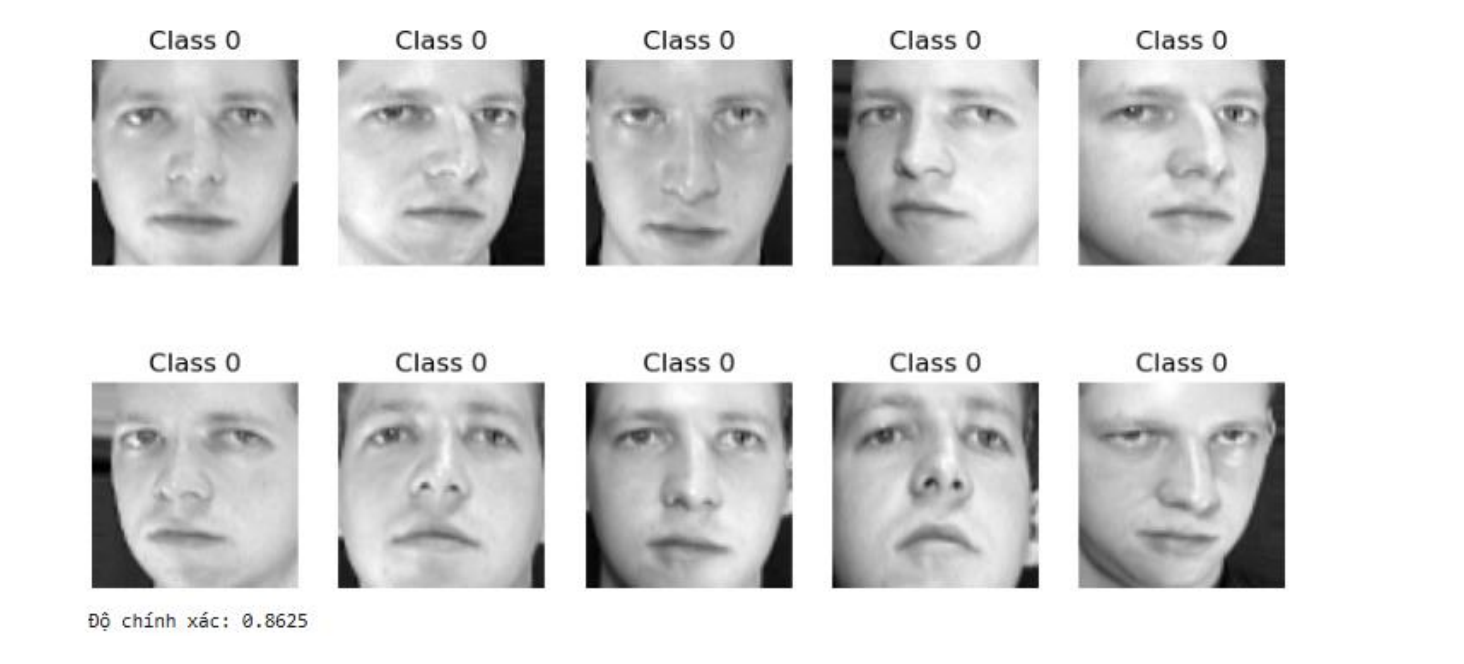
\includegraphics[scale=0.6]{img/10 khuon mat.png}
    \caption{Các hình ảnh khuôn mặt trong một lớp mẫu(Class 0)}
    \label{fig:enter-label}
\end{figure}
\begin{figure}[H]
    \centering
    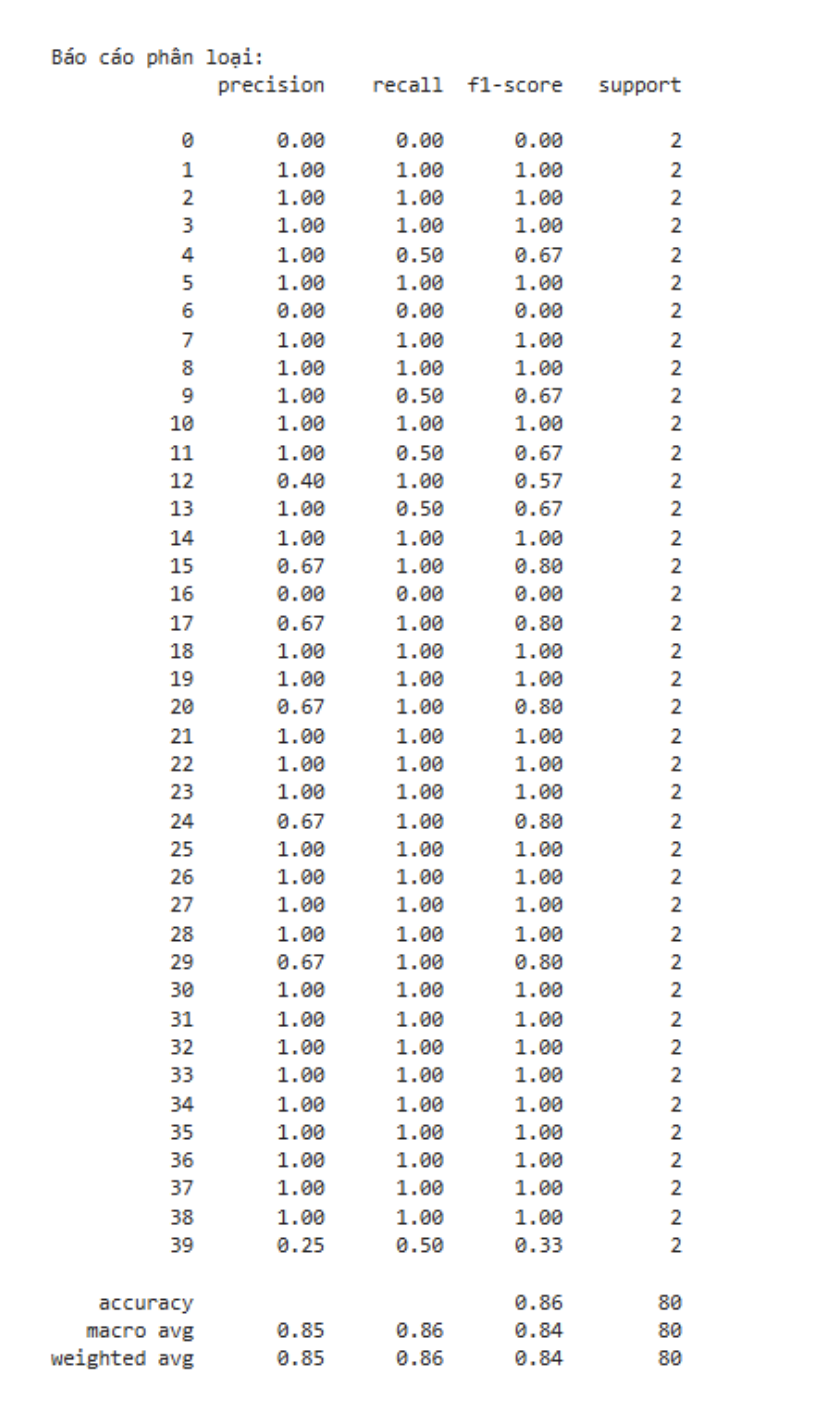
\includegraphics[scale=1]{img/baocaophanloai.png}
    \caption{Báo cáo phân loại và độ chính xác của mô hình}
    \label{fig:enter-label}
\end{figure}
\begin{figure}[H]
    \centering
    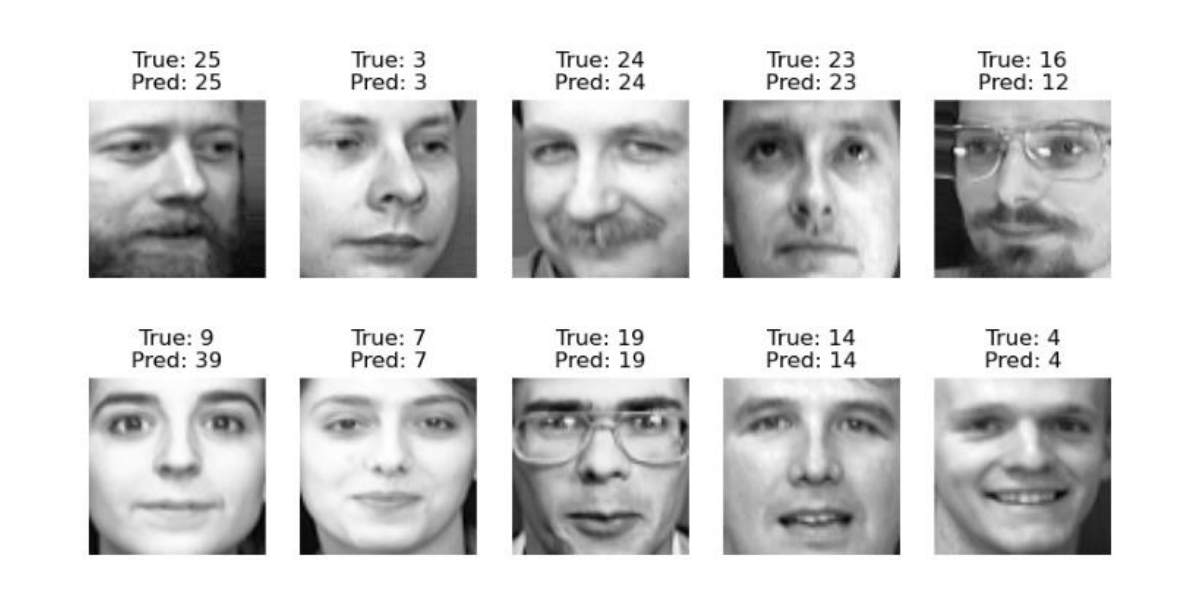
\includegraphics[scale=0.8]{img/ketquadudoanvanhanthucte.png}
    \caption{Kết quả dự đoán và nhãn thực tế}
    \label{fig:enter-label}
\end{figure}
\begin{figure}[h]
    \centering
    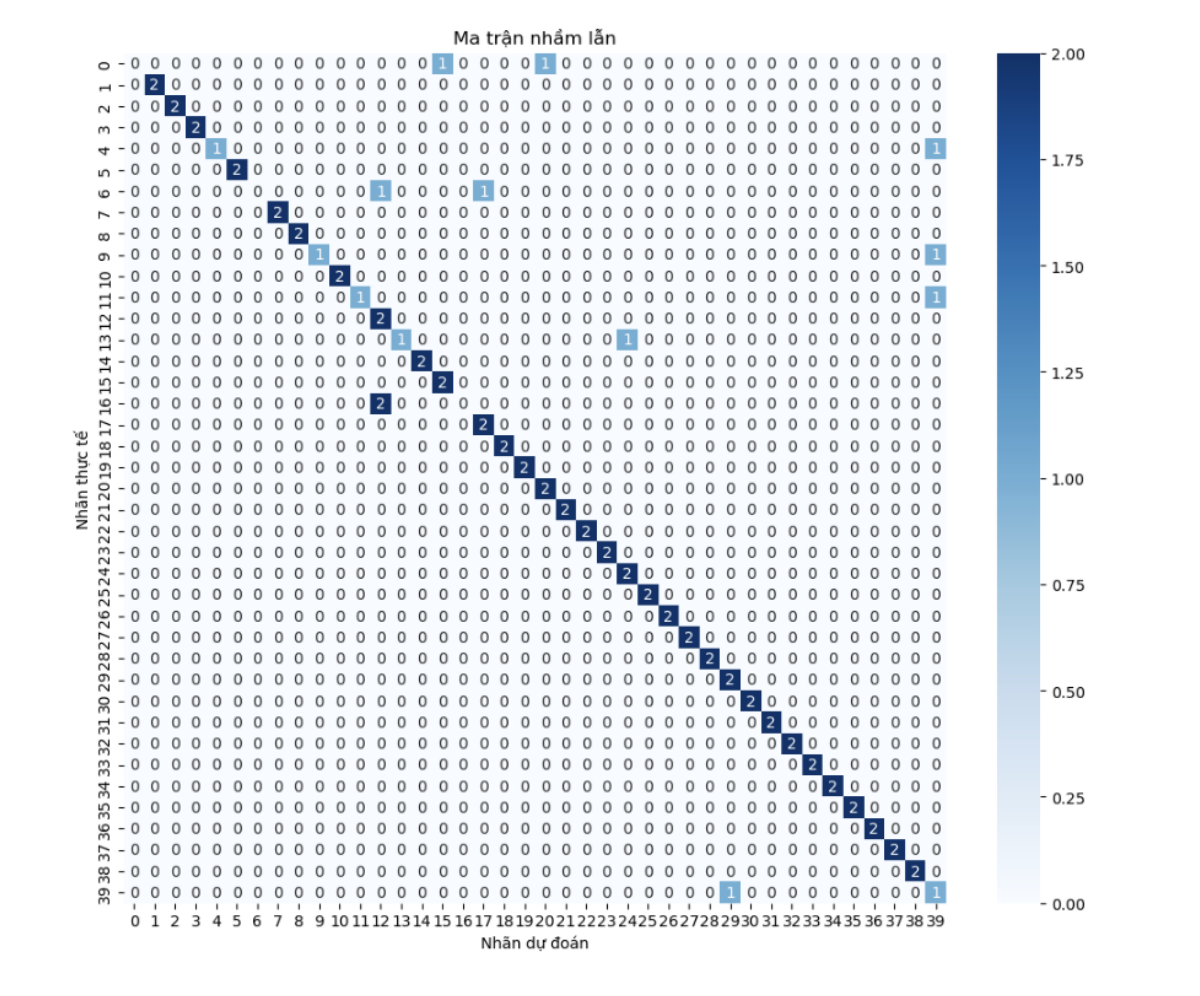
\includegraphics[scale=0.7]{img/Matrannhamlan.png}
    \caption{Ma trận nhầm lẫn}
    \label{fig:enter-label}
\end{figure}
\subsection{Kết quả và đánh giá}
{\large \textbf{Kết quả mô phỏng}}
\begin{itemize}
    \item Độ chính xác (Accuracy): Mô hình đạt độ chính xác khoảng 86.25\%, cho thấy mô hình có khả năng nhận diện khuôn mặt tốt trong điều kiện dữ liệu đã được tiền xử lý và thêm nhiễu.
    \item Báo cáo phân loại (Classification Report): Precision, Recall, và F1-Score dao động giữa các lớp:
    \begin{itemize}
        \item Một số lớp có F1-Score đạt gần 1.0 (ví dụ: các lớp 1, 2, 14), cho thấy mô hình nhận diện chính xác và ổn định cho các lớp này.
        \item  Một số lớp có F1-Score thấp (ví dụ: lớp 0, lớp 16, lớp 39), điều này phản ánh rằng mô hình gặp khó khăn khi nhận diện các khuôn mặt trong các lớp này.
    \end{itemize}
    \item Ma trận nhầm lẫn (Confusion Matrix): Cho thấy hầu hết các lớp được nhận diện đúng, nhưng vẫn tồn tại các trường hợp nhầm lẫn, đặc biệt là ở các lớp có đặc trưng không rõ ràng hoặc dễ bị ảnh hưởng bởi nhiễu.
\end{itemize}
{\large \textbf{Giải thích kết quả}}
\begin{enumerate}
    \item Độ chính xác tổng thể:
    \begin{itemize}
        \item Độ chính xác 86.25\% là một kết quả chấp nhận được trong bài toán nhận diện khuôn mặt, đặc biệt khi dữ liệu được làm khó bằng cách thêm nhiễu Gaussian và giảm số lượng mẫu huấn luyện.
        \item  Mô hình vẫn duy trì khả năng phân biệt khá tốt giữa các lớp khuôn mặt nhờ sử dụng SVD để giảm chiều và Fisherface Method (LDA) để tối ưu hóa phân biệt giữa các lớp.
    \end{itemize}
    \item Sự dao động trong F1-Score:
    \begin{itemize}
        \item Các lớp đạt F1-Score cao thường là những lớp có đặc trưng khuôn mặt nổi bật hoặc ít chịu ảnh hưởng bởi nhiễu.
        \item Các lớp đạt F1-Score thấp có thể do đặc trưng khuôn mặt không đủ rõ ràng, dữ liệu huấn luyện ít, hoặc bị ảnh hưởng nhiều bởi nhiễu.
    \end{itemize}
    \item Nhầm lẫn giữa các lớp:
    \begin{itemize}
        \item Các lớp dễ nhầm lẫn thường có đặc trưng khuôn mặt tương tự nhau hoặc bị ảnh hưởng bởi nhiễu, làm giảm khả năng phân biệt của mô hình.
    \end{itemize}
\end{enumerate}
{\large \textbf{Đánh giá}}
\begin{itemize}
    \item \textbf{Ưu điểm của mô hình:}
    \begin{itemize}
        \item SVD giúp giảm chiều dữ liệu, loại bỏ nhiễu và giữ lại các đặc trưng quan trọng, làm dữ liệu dễ xử lý hơn.
        \item Fisherface Method (LDA): Tăng khả năng phân biệt giữa các lớp, đặc biệt trong bài toán nhiều lớp (40 lớp).
        \item Kết quả độ chính xác cao (86.25\%) cho thấy mô hình hoạt động tốt trên tập dữ liệu Olivetti Faces, một bộ dữ liệu chứa nhiều biến thể khuôn mặt.
    \end{itemize}
    \item \textbf{Hạn chế của mô hình:}
    \begin{itemize}
        \item Khi giảm số lượng mẫu huấn luyện (chỉ 5 ảnh/lớp) và thêm nhiễu Gaussian, mô hình gặp khó khăn hơn trong việc học đặc trưng, dẫn đến sự nhầm lẫn ở một số lớp.
        \item Độ chính xác không đồng đều giữa các lớp, cho thấy khả năng phân biệt không đồng nhất giữa các khuôn mặt.
    \end{itemize}
\end{itemize}

%Chapter 5 Kết luận
\section{Kết luận}
\subsection{Tóm tắt bài báo cáo}
Bài báo cáo đã tập trung triển khai ứng dụng phương pháp SVD (Singular Value Decomposition) và
Fisherface Method dựa trên LDA (Linear Discriminant Analysis) trong bài toán nhận diện khuôn mặt.
Các nội dung chính bao gồm:
\begin{itemize}
    \item Phần lý thuyết: Giới thiệu các khái niệm cơ bản về SVD, Fisherface Method và cách kết hợp hai phương pháp này trong nhận diện khuôn mặt.
    \item Phần thực hành: Xây dựng quy trình mô phỏng bằng Python, từ tiền xử lý dữ liệu, giảm chiều bằng SVD, phân loại bằng Fisherface Method, đến đánh giá hiệu quả mô hình.
    \item Kết quả đạt được: Mô hình đạt độ chính xác trung bình 86.25\%, thể hiện khả năng nhận diện khuôn mặt tốt trong điều kiện dữ liệu giả lập và được làm khó bằng nhiễu Gaussian.
\end{itemize}
\subsection{Những hoạt động trong bài báo cáo}
\begin{enumerate}
    \item Lý thuyết:
    \begin{itemize}
        \item Trình bày cơ sở lý thuyết của phương pháp SVD và Fisherface Method, bao gồm cách sử dụng SVD để giảm chiều dữ liệu và Fisherface Method để tối ưu hóa khả năng phân biệt giữa các lớp khuôn mặt.
        \item Phân tích ưu điểm và nhược điểm của hai phương pháp, cũng như lý do kết hợp chúng trong bài toán nhận diện khuôn mặt.
    \end{itemize}
    \item Thực hành:
    \begin{itemize}
        \item Sử dụng bộ dữ liệu Olivetti Faces để mô phỏng bài toán nhận diện khuôn mặt. Viết mã Python với sự hỗ trợ của các thư viện như NumPy, scikit-learn và Matplotlib để thực hiện quy trình từ tiền xử lý dữ liệu, giảm chiều, phân loại đến đánh giá.
        \item Hiển thị kết quả trực quan, bao gồm các hình ảnh mẫu, ma trận nhầm lẫn và báo cáophân loại.
    \end{itemize}
    \item Kết quả đạt được:
    \begin{itemize}
        \item Mô hình đạt độ chính xác 86.25\%, với sự dao động về hiệu suất giữa các lớp. Một số lớp được nhận diện chính xác cao, trong khi một số lớp gặp khó khăn do nhiễu hoặc thiếu đặc trưng nổi bật.
    \end{itemize}
\end{enumerate}
\subsection{Hạn chế và bài học}
\begin{enumerate}
    \item Hạn chế:
    \begin{itemize}
        \item Dữ liệu nhỏ: Bộ dữ liệu Olivetti Faces chỉ bao gồm 400 hình ảnh và 40 lớp, nên chưa thể mô phỏng đầy đủ các tình huống thực tế.
        \item Nhiễu ảnh hưởng đến hiệu suất: Việc thêm nhiễu Gaussian khiến mô hình gặp khó khăn trong việc học đặc trưng, đặc biệt với các lớp có ít mẫu hoặc không nổi bật.
        \item Hiệu suất không đồng đều: Một số lớp có F1-Score thấp, phản ánh rằng mô hình chưa xử lý tốt với dữ liệu có đặc trưng gần giống nhau.
    \end{itemize}
    \item Bài học để rút kinh nghiệm:
    \begin{itemize}
        \item Sự kết hợp giữa SVD và Fisherface Method là một phương pháp phù hợp trong bài toán nhận diện khuôn mặt, đặc biệt khi dữ liệu nhỏ và cần tối ưu hóa việc phân loại.
        \item Việc chuẩn bị dữ liệu và tiền xử lý đóng vai trò quan trọng trong việc nâng cao hiệu quả của mô hình.
    \end{itemize}
\end{enumerate}
\subsection{Kết luận cuối cùng}
Bài báo cáo đã thực hiện thành công việc triển khai và đánh giá hiệu quả của phương pháp SVD và Fisherface Method trong bài toán nhận diện khuôn mặt. Mặc dù có một số hạn chế, mô hình đã cho thấy kết quả khả quan với độ chính xác cao trong điều kiện dữ liệu giả lập. \\
Các kết quả đạt được từ bài báo cáo này không chỉ minh họa được lý thuyết mà còn cung cấp một
quy trình thực hành chi tiết, giúp nhóm hiểu rõ hơn về cách áp dụng các thuật toán trong thị giác máy tính. Đây sẽ là cơ sở để nhóm tiếp tục nghiên cứu, cải thiện và áp dụng vào các bài toán tương tự trong tương lai.
\newpage
\section{Tài liệu tham khảo}
[1] G. H. Golub and C. F. Van Loan, {\textit{Matrix Computations}, 4th ed., Johns Hopkins University Press, 2013. \\
$[2]$ P. N. Belhumeur, J. P. Hespanha, and D. J. Kriegman, “Eigenfaces vs. Fisherfaces: Recognition using class specific linear projection,” {\textit{IEEE Transactions on Pattern Analysis and Machine}, 1997. \\
$[3]$ J. Shlens, “A tutorial on principal component analysis,” {\textit{arXiv preprint arXiv:1404.1100}, 2014. \\
$[4]$ R. Chellappa, C. L. Wilson, and S. Sirohey, “Human and machine recognition of faces: A survey,” {\textit{Proceedings of the IEEE}, 1995. \\
\end{document}